\chapter{Software Design}

\section{Introduction to Software Design}

This chapter presents the detailed software design of the Property Rental System platform. It translates the requirements identified in Chapter~3 into structured architectural, behavioural, and data models. The purpose of this chapter is to provide a clear blueprint for system implementation, ensuring maintainability, scalability, and modular development.

The chapter covers the design methodology and software process model, a high-level system overview and architecture, UML behavioural and structural models, data flow diagrams, and the database design including the entity relationship model, schema, and data dictionary for the platform's MongoDB collections.

%%%%%%%%%%%%%%%%%%%%%%%%%%%%%%%%%%%%%%%%%%%%%%%%%%%%%%
\section{Design Methodology and Software Process Model}

\subsection{Design Methodology}

Property Rental System follows an object-oriented, layered design methodology combined with the Model-View-Controller pattern on the backend. The system is divided into a presentation layer (React client), an application layer (Express controllers and services), and a data layer (MongoDB through Mongoose models). Within the application layer, controllers handle request and response concerns while services encapsulate business logic, giving a clear separation of concerns.

This methodology was selected because it suits a web application with multiple user roles and evolving features. It enforces loose coupling between layers, promotes reuse of services across controllers, and allows each module to be developed and tested independently. The design adheres to established principles including Separation of Concerns, the DRY (Don't Repeat Yourself) principle, and SOLID object-oriented design guidelines, particularly single-responsibility services and dependency inversion through well-defined interfaces.

\subsection{Software Process Model}

The project follows the \textbf{Agile (iterative and incremental)} process model. Agile was selected because the requirements were refined progressively through stakeholder feedback and supervisor reviews, and because the platform's features, such as listing management, search, booking, and roommate matching, lend themselves naturally to incremental delivery. Development proceeded in short iterations, each delivering a working slice of functionality that was tested and reviewed before the next iteration began. Testing and validation were integrated continuously rather than deferred to a single final phase, allowing defects to be identified and corrected early.

%%%%%%%%%%%%%%%%%%%%%%%%%%%%%%%%%%%%%%%%%%%%%%%%%%%%%%
\section{System Overview}

This section provides a high-level overview of the system components and their interactions with external entities. At the boundary, three human actors, the tenant, the landlord, and the administrator, interact with the Property Rental System platform, while three external services, the Google Maps API, cloud media storage, and the email service, support the platform's operation. The context diagram below depicts the system as a single process exchanging data with these external entities.

\begin{figure}[h]
\centering
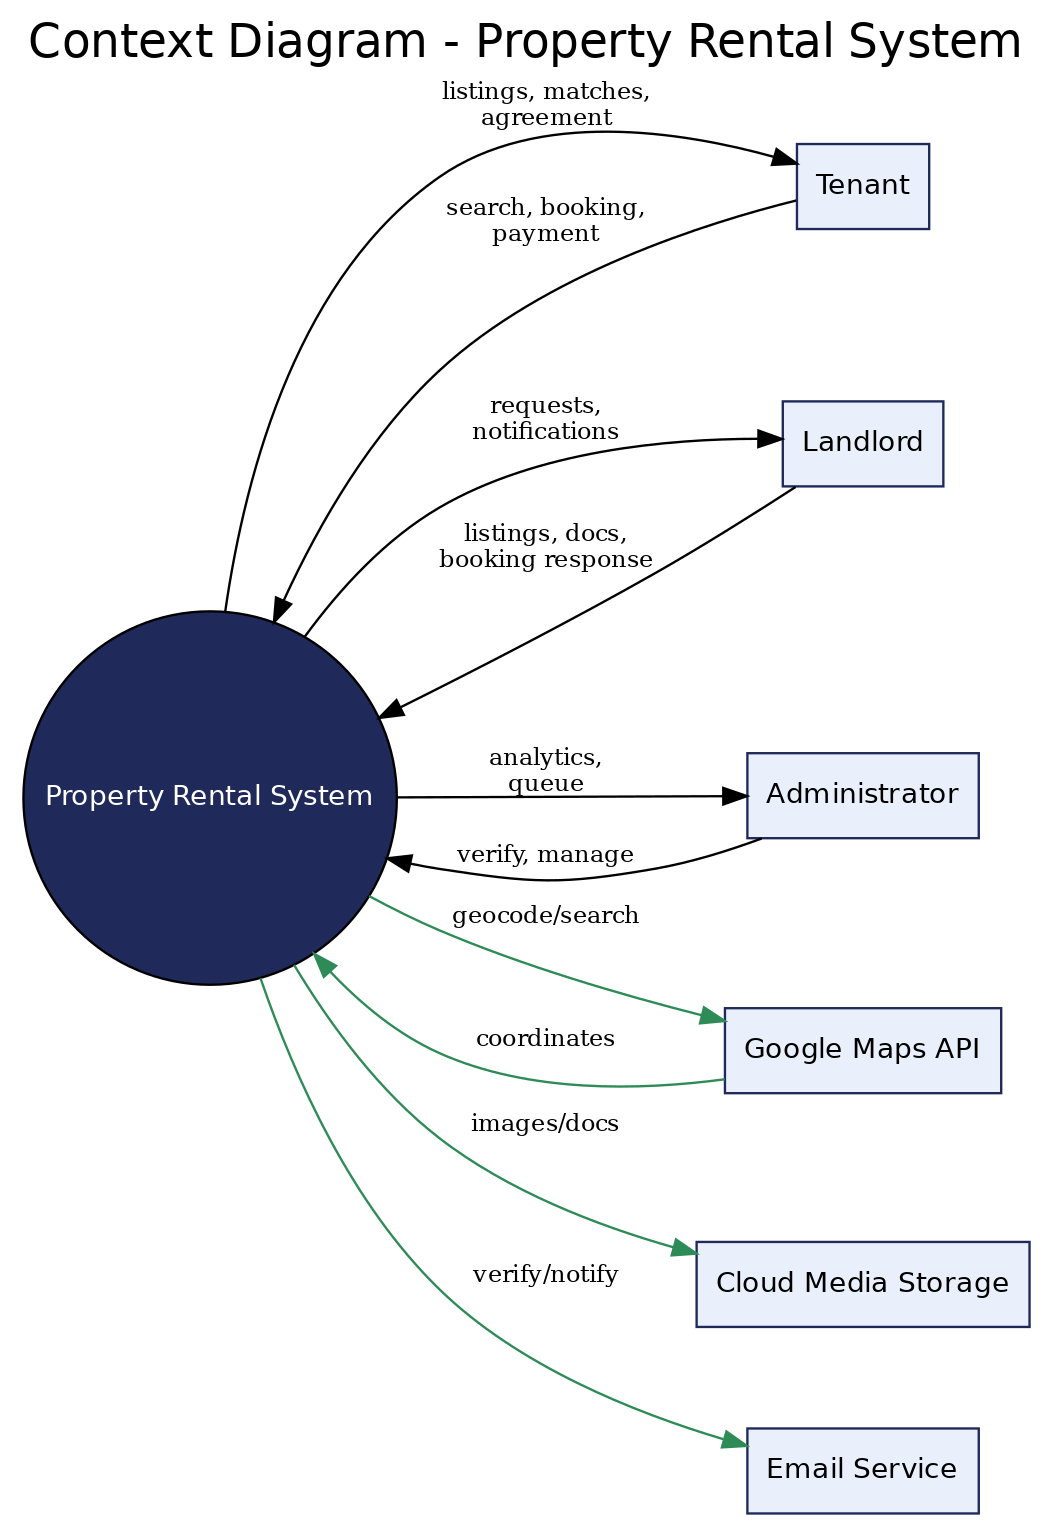
\includegraphics[width=0.9\textwidth]{Figures/Context Diagram.png}
\caption{Context Diagram of the Property Rental System Platform}
\label{fig:context}
\end{figure}

\noindent\textit{(The figure above is a sample from the template; replace it with the finalised Property Rental System context diagram before submission.)} The diagram shows the system boundary, the human actors who submit requests and receive responses, and the third-party services that the platform calls for mapping, storage, and email.

%%%%%%%%%%%%%%%%%%%%%%%%%%%%%%%%%%%%%%%%%%%%%%%%%%%%%%
\section{Architectural Design}

Property Rental System adopts a three-layer client-server architecture. The presentation layer is a React single-page application built with Vite and styled with Tailwind CSS, using Zustand for client-side state. It communicates with the backend solely through a RESTful API over HTTPS. The application layer is a Node.js and Express.js server organised into routes, controllers, and services; it enforces authentication and role-based access control through middleware and implements all business logic in dedicated service classes such as the authentication, property, booking, payment, chat, agreement, and roommate-matching services. The data layer is a MongoDB database accessed through Mongoose models, complemented by external integrations for geospatial search, media storage, and email.

\begin{figure}[h]
\centering
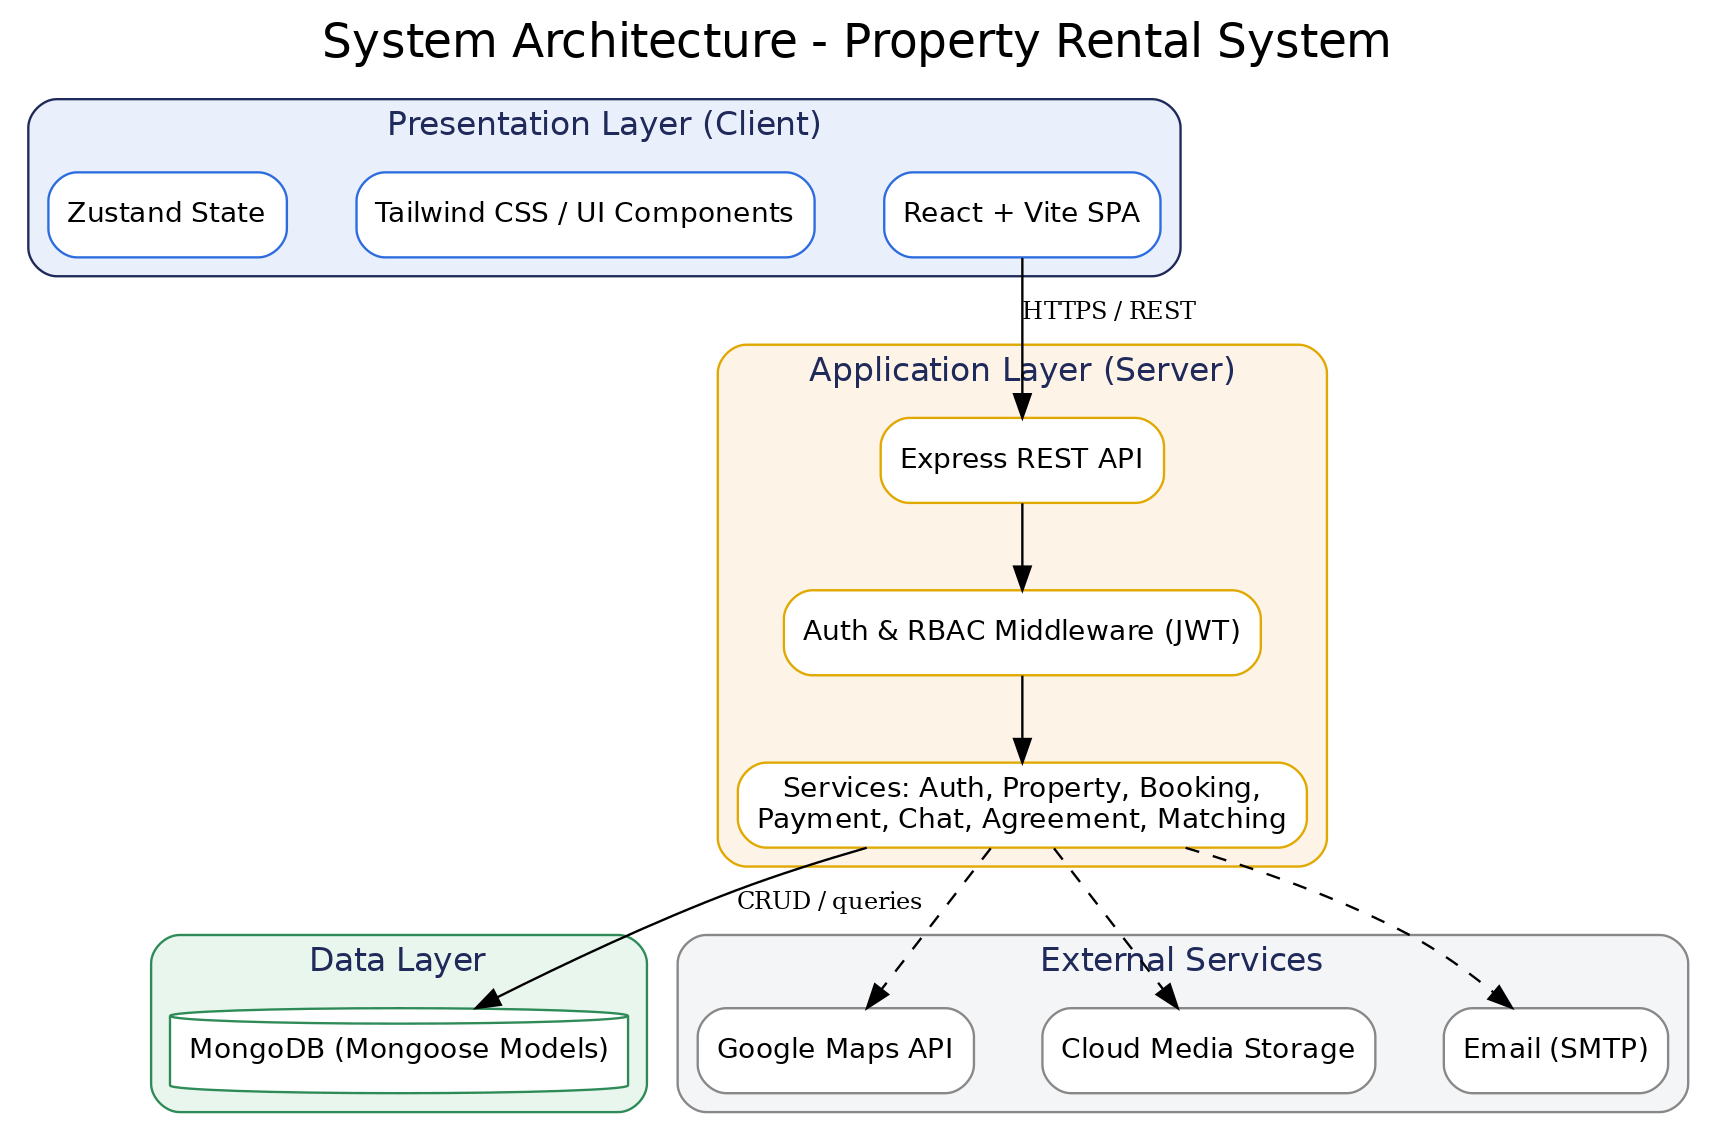
\includegraphics[width=0.9\textwidth]{Figures/Architecture Diagram.png}
\caption{System Architecture of the Property Rental System Platform}
\label{fig:arch}
\end{figure}

\noindent\textit{(Sample template figure; replace with the finalised Property Rental System architecture diagram.)} The presentation layer issues API requests; the API layer authenticates and authorises each request, delegates to the appropriate service, and the service interacts with the data layer and external services. Responses flow back through the same layers, keeping the frontend decoupled from data and integration concerns.

%%%%%%%%%%%%%%%%%%%%%%%%%%%%%%%%%%%%%%%%%%%%%%%%%%%%%%
\section{Design Models}

This section presents detailed design models describing system behaviour, structure, and interactions using UML diagrams. These models help developers understand the system workflow before implementation.

%%%%%%%%%%%%%%%%%%%%%%%%%%%%%%%%%%%%%%%%%%%%%%%%%%%%%%
\subsection{Activity Diagrams}

Activity diagrams represent the workflow of the major modules of the platform. Each core module is described by a separate activity diagram capturing user interaction, validation checks, decision points, and database interaction.

\begin{figure}[h]
\centering
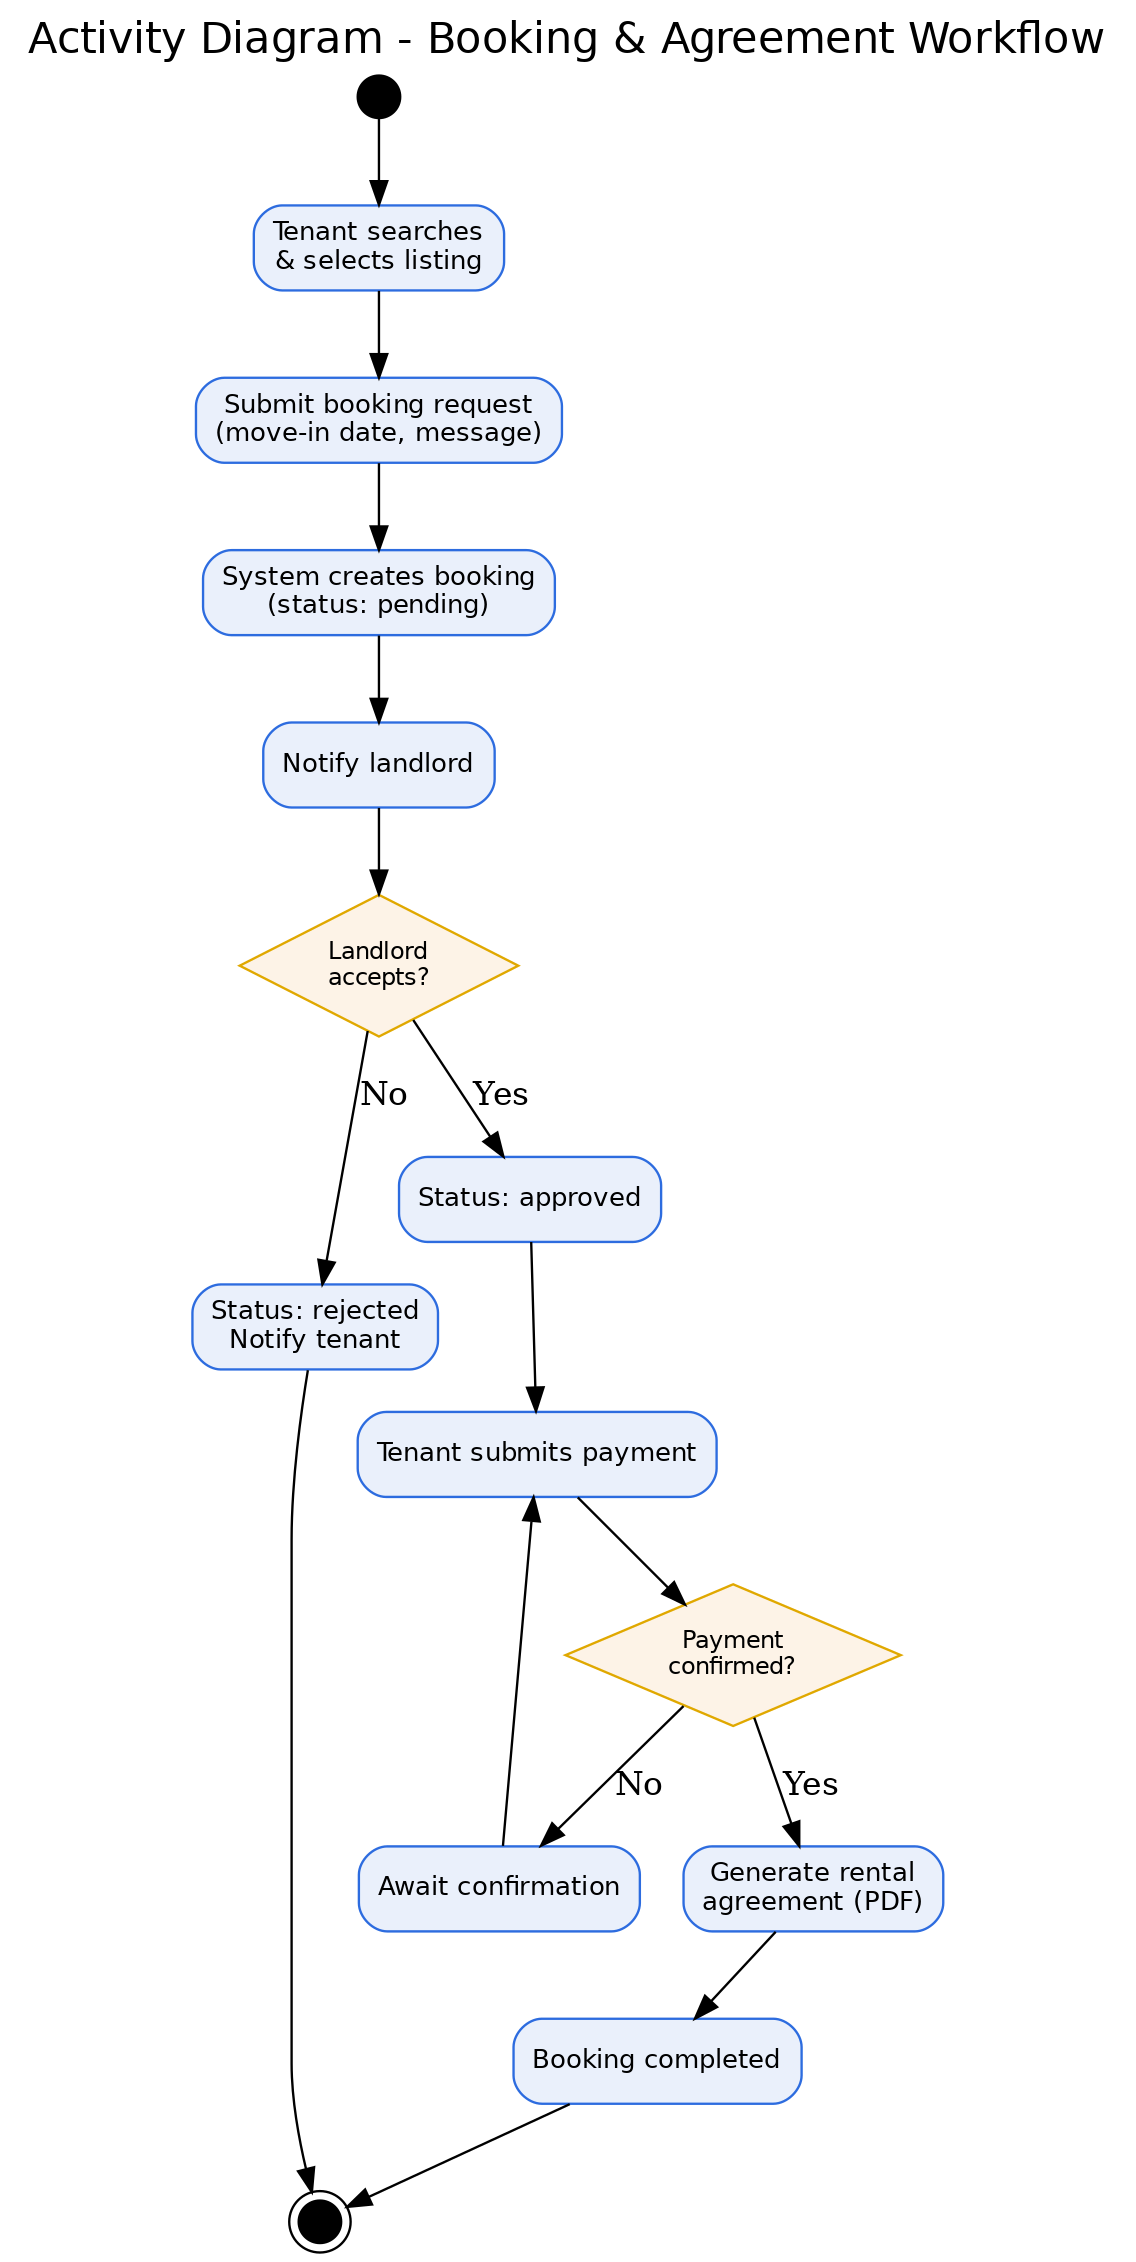
\includegraphics[width=0.67\textwidth]{Figures/Activity Diagram.png}
\caption{Activity Diagram (Sample)}
\label{fig:activity}
\end{figure}

\subsubsection{Module 1: User Management}

This activity diagram illustrates the registration, login, and verification workflow. The flow begins with the user submitting credentials, proceeds through input validation, account creation, and email verification, and includes a decision point where unverified accounts are restricted from protected actions until verification completes.

\subsubsection{Module 2: Property Listing and Booking}

This activity diagram captures the core rental workflow: a landlord creates a listing, the listing awaits verification, a tenant searches and submits a booking request, the landlord accepts or rejects it, payment is recorded, and a digital agreement is generated. Decision nodes handle validation failures, rejected bookings, and unconfirmed payments.

\subsubsection{Module 3: Admin Module}

This activity diagram describes administrator operations, including reviewing verification requests, approving or rejecting documents, managing user status, confirming payments, and viewing analytics.

%%%%%%%%%%%%%%%%%%%%%%%%%%%%%%%%%%%%%%%%%%%%%%%%%%%%%%
\subsection{Class Diagram}

The class diagram shows the static structure of the system, including the principal domain classes, their attributes, and their relationships.

\begin{figure}[h]
\centering
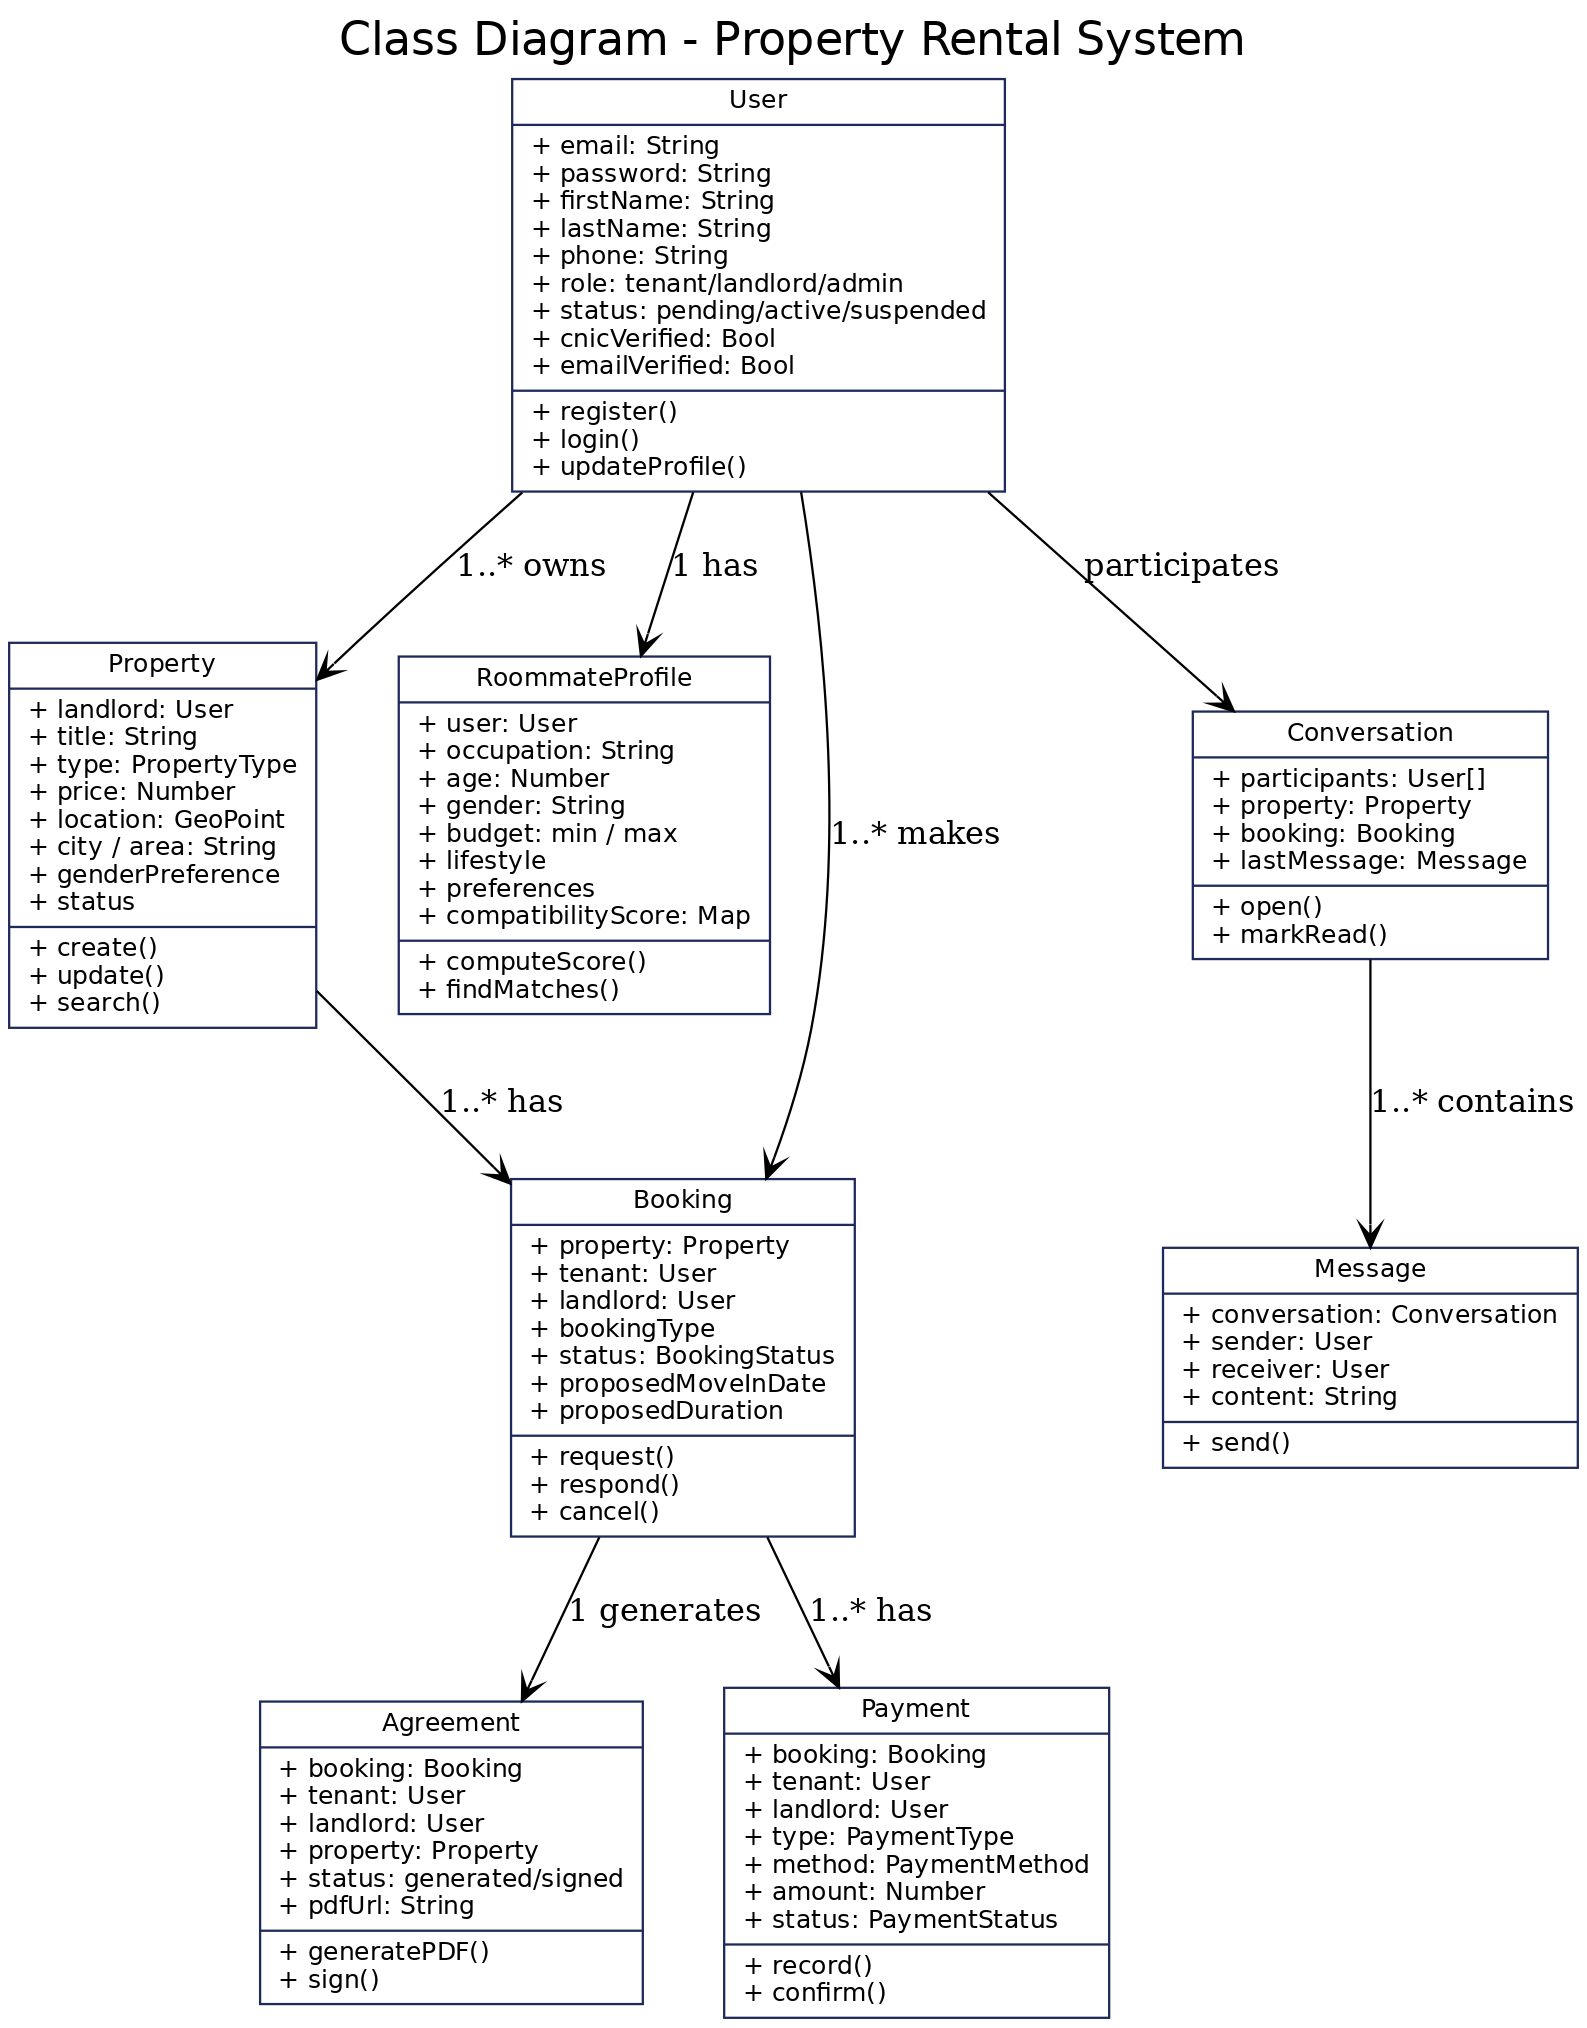
\includegraphics[width=0.88\textwidth]{Figures/Class Diagram.png}
\caption{Class Diagram (Sample)}
\label{fig:class}
\end{figure}

The key classes of Property Rental System are \texttt{User} (with subtypes distinguished by role), \texttt{Property}, \texttt{RoommateProfile}, \texttt{Booking}, \texttt{Agreement}, \texttt{Payment}, \texttt{Conversation}, \texttt{Message}, \texttt{Document}, and \texttt{LandlordBankAccount}. A \texttt{User} acting as a landlord owns many \texttt{Property} listings; a \texttt{User} acting as a tenant creates many \texttt{Booking} records; each \texttt{Booking} relates one tenant, one landlord, and one property and may generate one \texttt{Agreement} and one or more \texttt{Payment} records. \texttt{Conversation} aggregates many \texttt{Message} objects between two users. Each \texttt{User} may have one \texttt{RoommateProfile}, which the matching service uses to compute compatibility. These relationships include association, aggregation, and role-based specialisation.

%%%%%%%%%%%%%%%%%%%%%%%%%%%%%%%%%%%%%%%%%%%%%%%%%%%%%%
\subsection{Sequence Diagrams}

Sequence diagrams show the interaction between objects over time, including the request-response flow between the actor, the system components, and the database.

\subsubsection{Sequence Diagram -- User Login}

\begin{figure}[h]
\centering
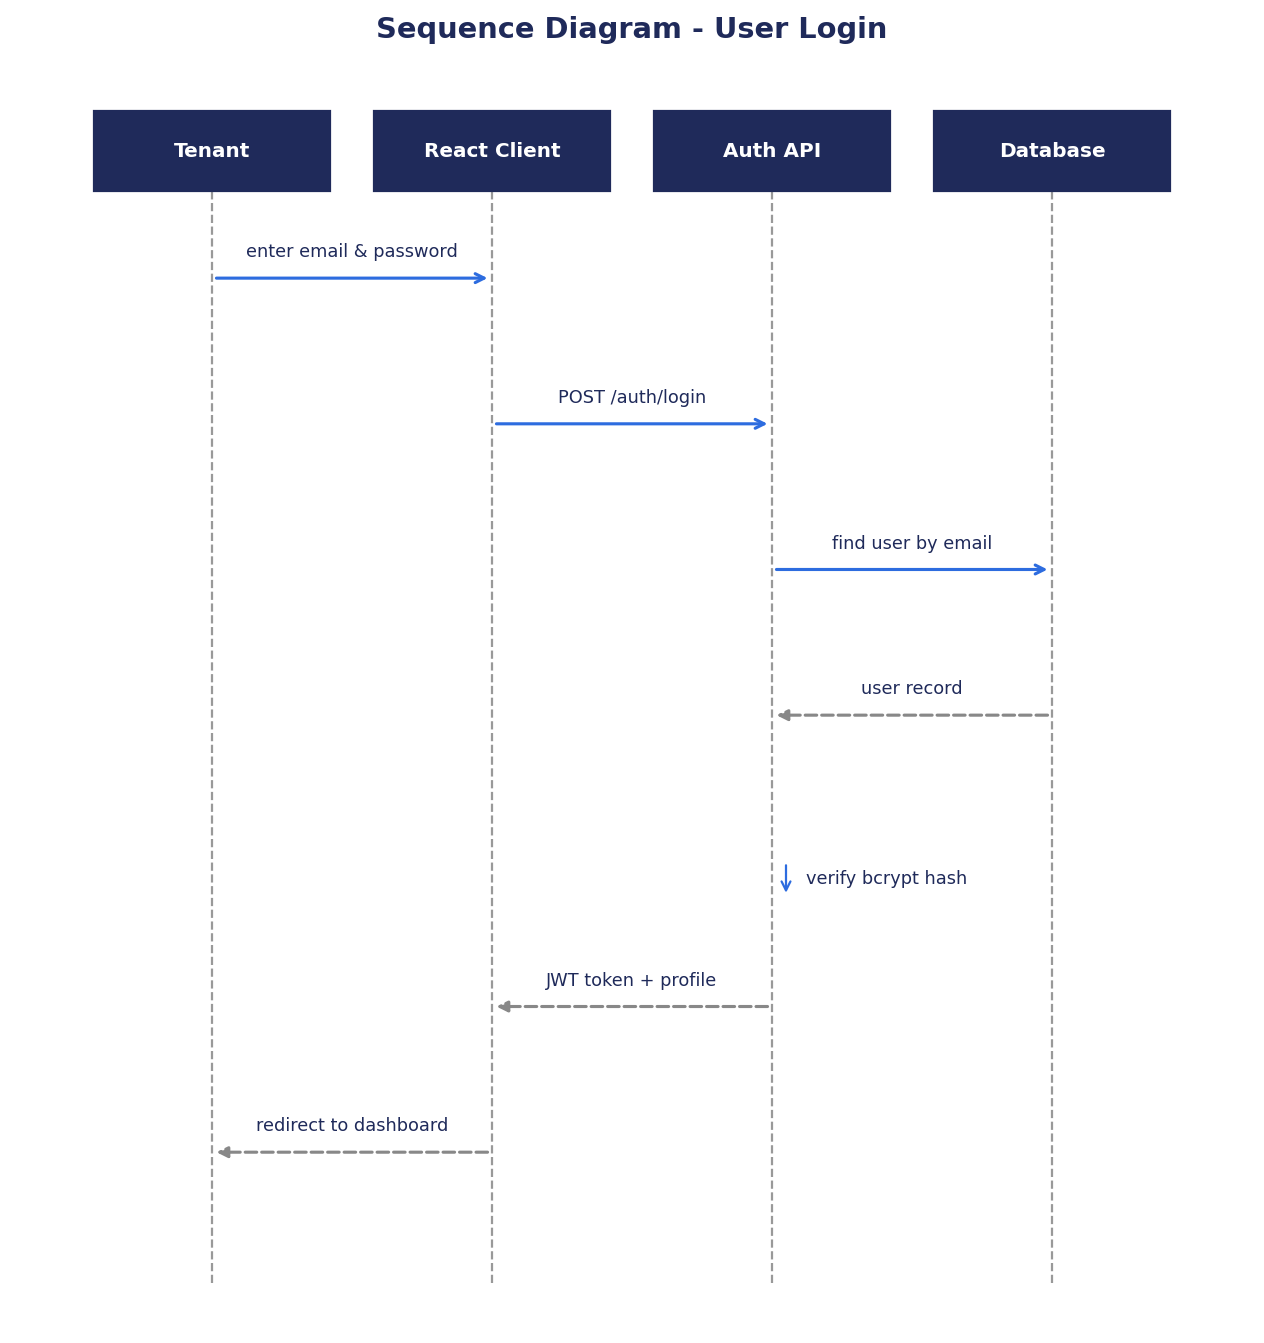
\includegraphics[width=0.8\textwidth]{Figures/Sequence Diagram 2.png}
\caption{Sequence Diagram -- User Login (Sample)}
\label{fig:seq1}
\end{figure}

In the login sequence, the user submits credentials to the React client, which sends them to the authentication endpoint. The authentication service validates the credentials against the user record in MongoDB, verifies the hashed password, issues a JWT on success, and returns it to the client, which stores it for subsequent authenticated requests.

\subsubsection{Sequence Diagram -- Booking and Agreement}

\begin{figure}[h]
\centering
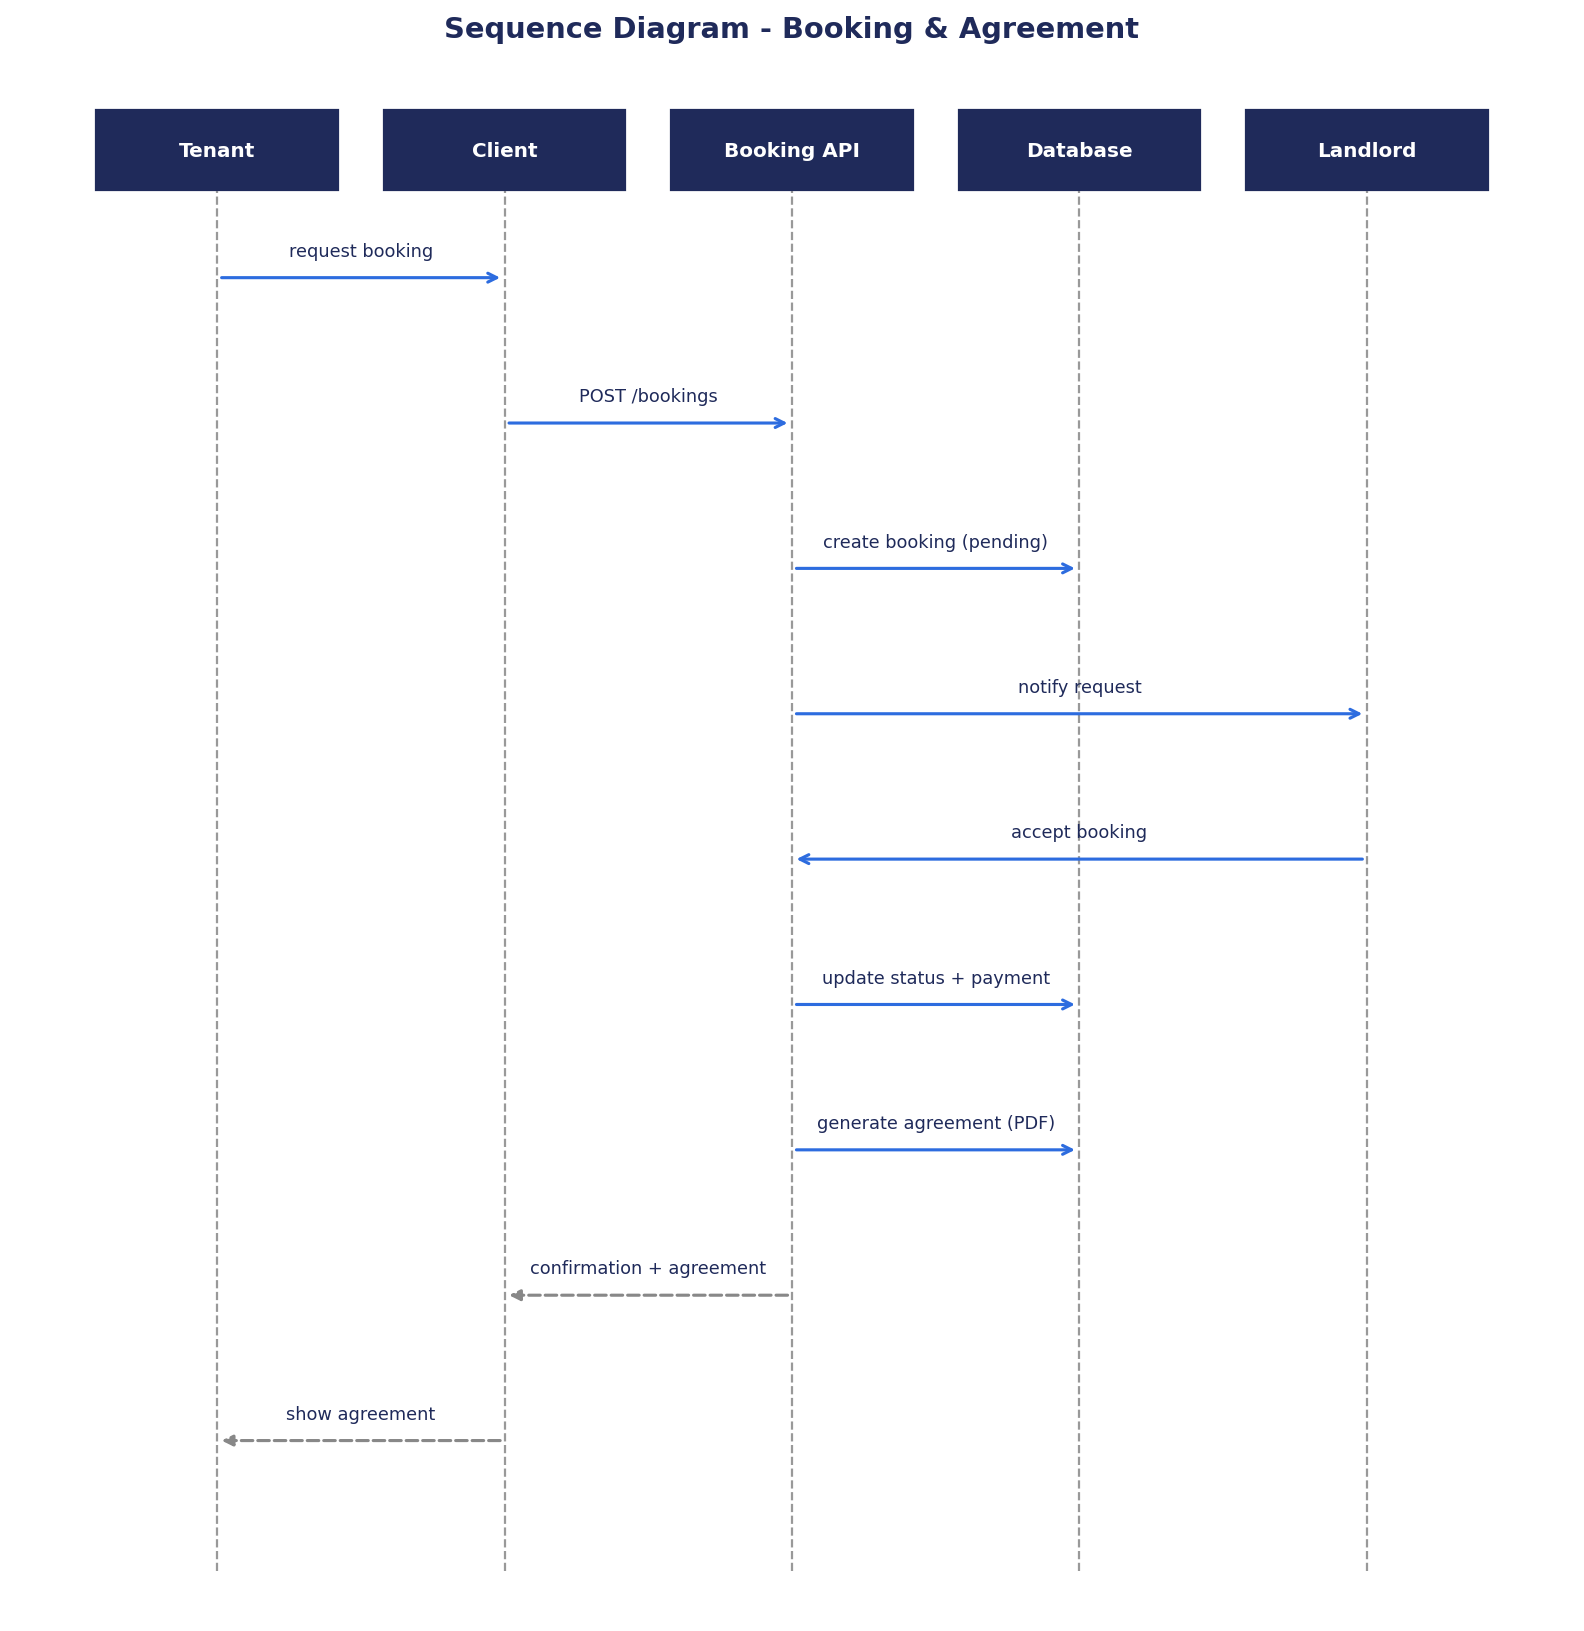
\includegraphics[width=0.8\textwidth]{Figures/Sequence Diagram.png}
\caption{Sequence Diagram -- Booking and Agreement (Sample)}
\label{fig:seq2}
\end{figure}

In the booking sequence, the tenant submits a booking request; the booking service creates a pending booking and notifies the landlord; upon acceptance and confirmed payment, the agreement service generates a PDF rental agreement and persists it, after which both parties are notified.

%%%%%%%%%%%%%%%%%%%%%%%%%%%%%%%%%%%%%%%%%%%%%%%%%%%%%%
\subsection{State Transition Diagrams}

\begin{figure}[h]
\centering
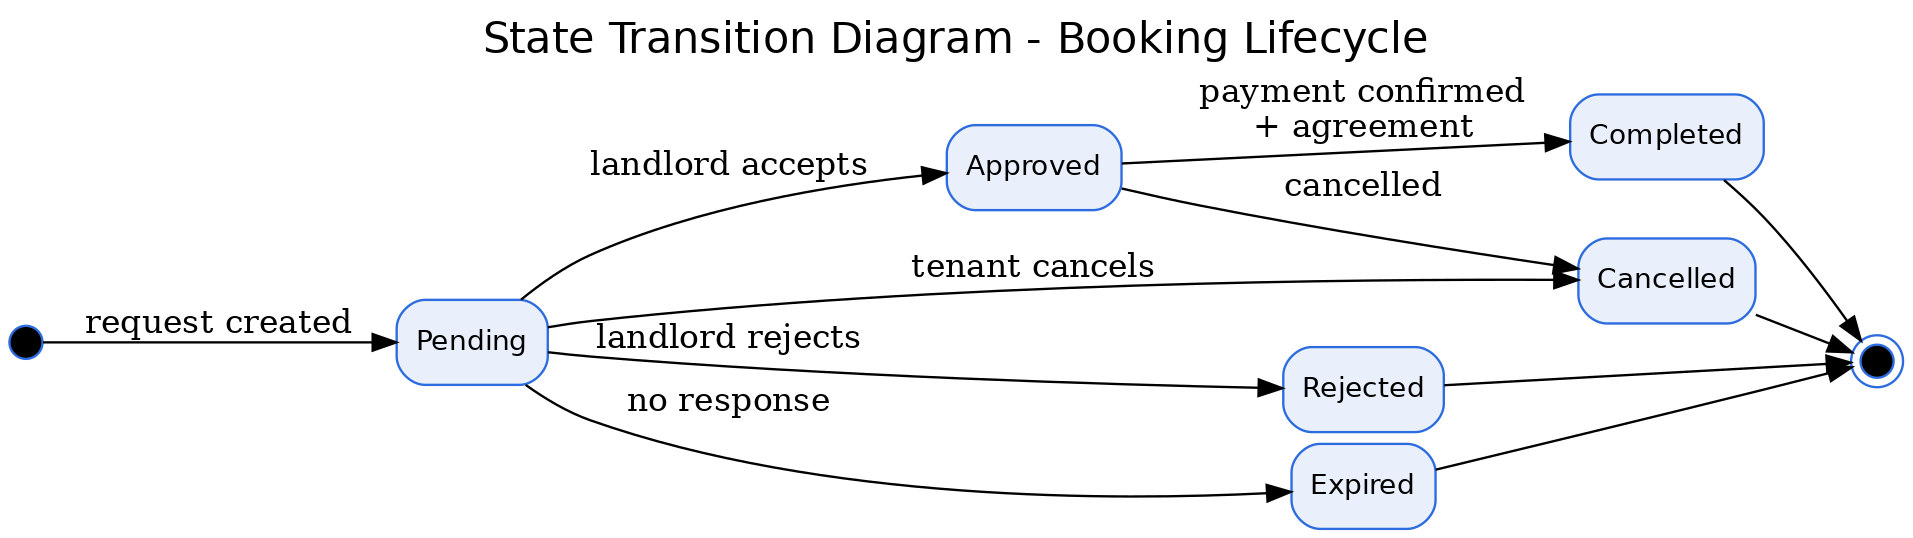
\includegraphics[width=0.77\textwidth]{Figures/State Transition.png}
\caption{State Transition Diagram (Sample)}
\label{fig:state}
\end{figure}

State transition diagrams show how key entities change state over their lifecycle. Two important examples in Property Rental System are the user account and the booking. A \textbf{User account} transitions through the states \textit{Pending} (just registered), \textit{Active} (verified), and \textit{Suspended} (administratively blocked). A \textbf{Booking} transitions through \textit{Pending} (requested), \textit{Accepted} or \textit{Rejected} (landlord decision), \textit{Confirmed} (payment recorded), and \textit{Completed} or \textit{Cancelled}. A \textbf{Property} listing transitions through \textit{Pending Verification}, \textit{Active}, and \textit{Inactive}. Each transition is triggered by a specific event, such as approval, payment, or administrative action.

%%%%%%%%%%%%%%%%%%%%%%%%%%%%%%%%%%%%%%%%%%%%%%%%%%%%%%
\section{Data Flow Diagrams}

Data Flow Diagrams describe how data moves within the system. Different levels provide increasing detail.

\subsection{Level 1 Data Flow Diagram}

\begin{figure}[h]
\centering
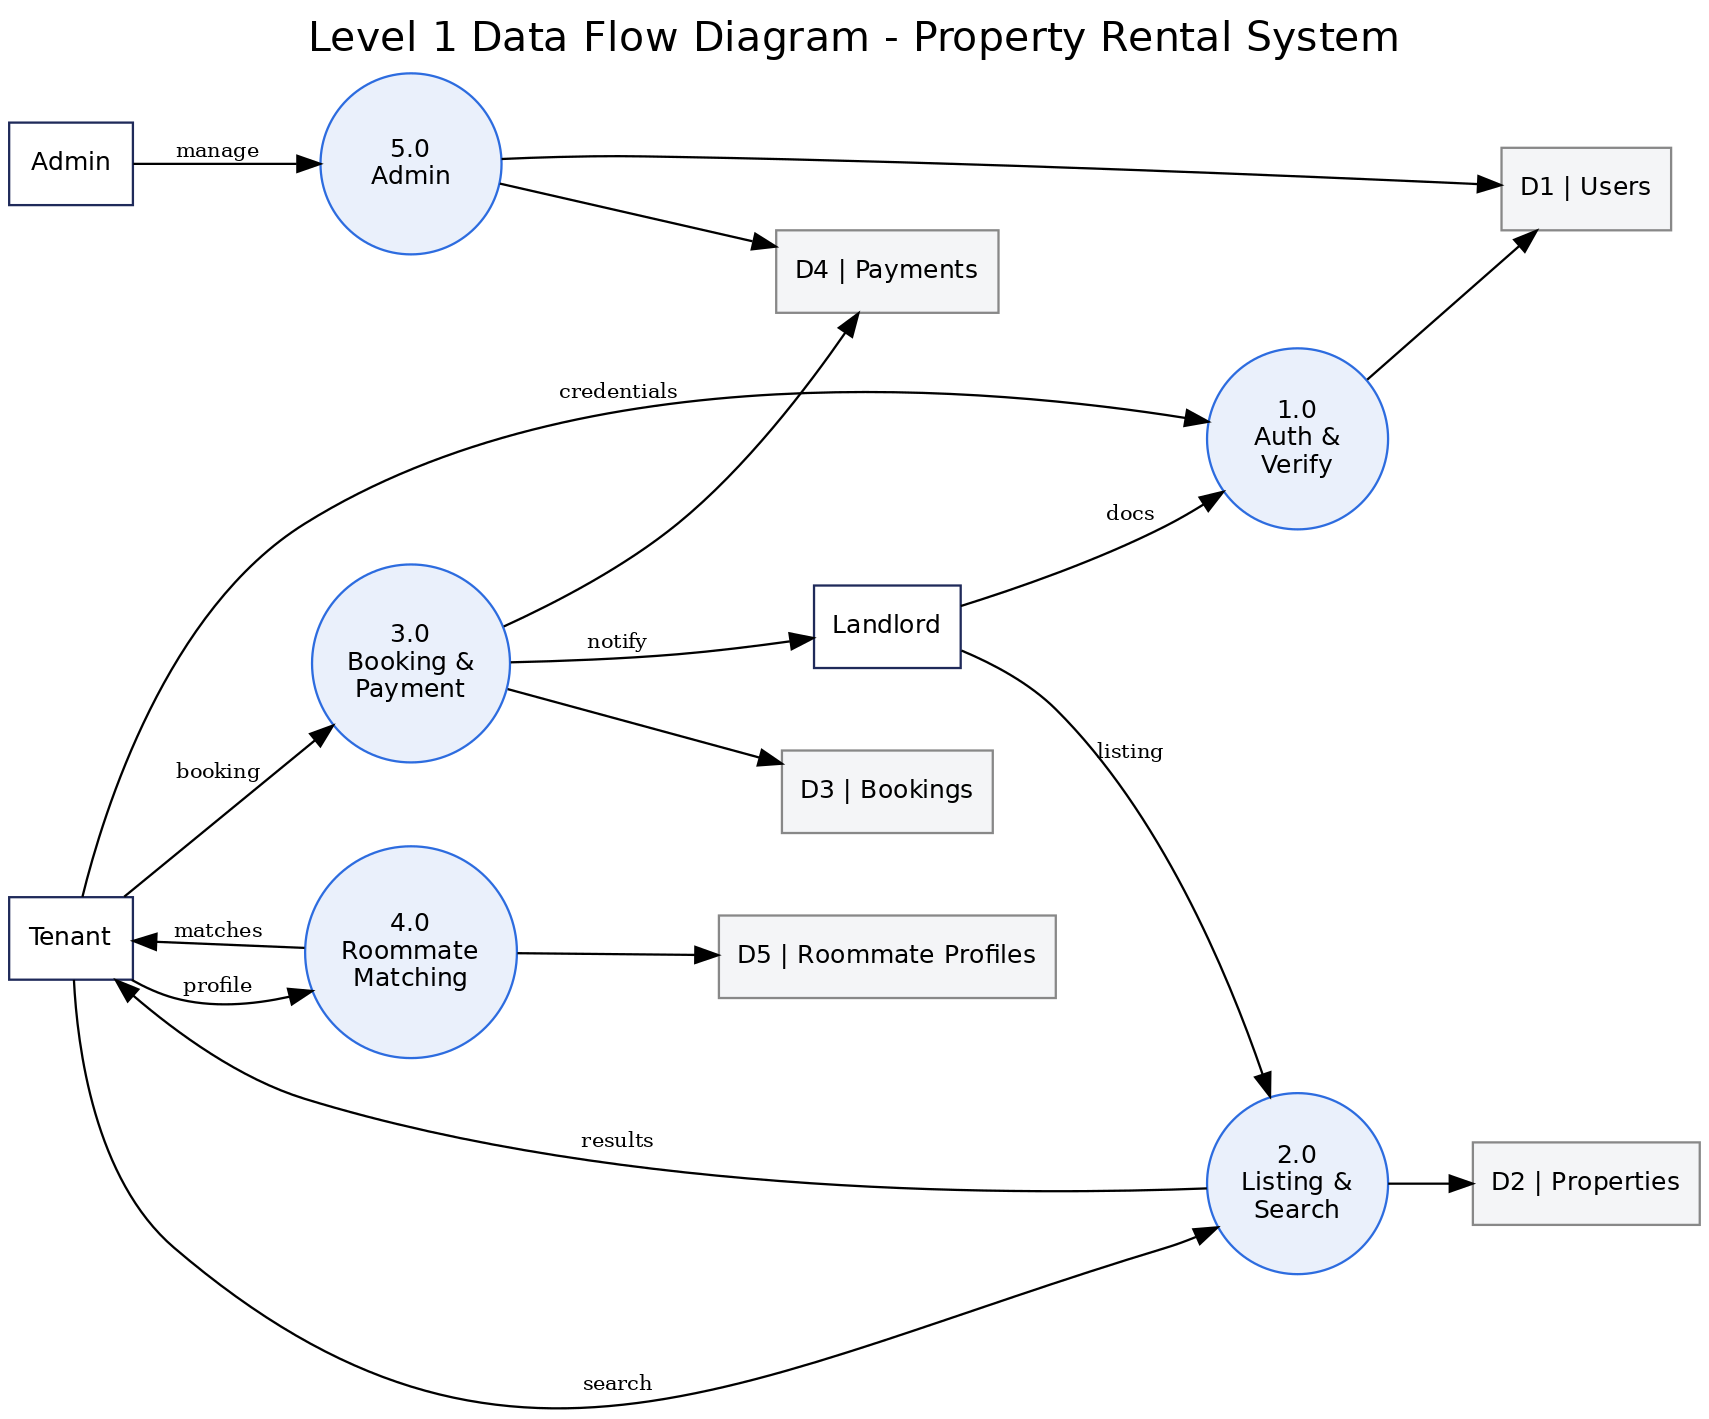
\includegraphics[width=0.9\textwidth]{Figures/DFD Sample.png}
\caption{Level 1 Data Flow Diagram (Sample)}
\label{fig:dfd1}
\end{figure}

The Level 1 DFD decomposes the platform into its major sub-processes: the Authentication and Verification process, the Property Listing and Search process, the Booking and Payment process, the Roommate Matching process, and the Administration process. Each process exchanges data with the relevant data stores, namely the Users, Properties, Bookings, Payments, Agreements, and Roommate Profiles collections, while external entities (tenant, landlord, administrator) provide inputs and receive outputs.

\subsection{Level 2 Data Flow Diagram}

\begin{figure}[h]
\centering
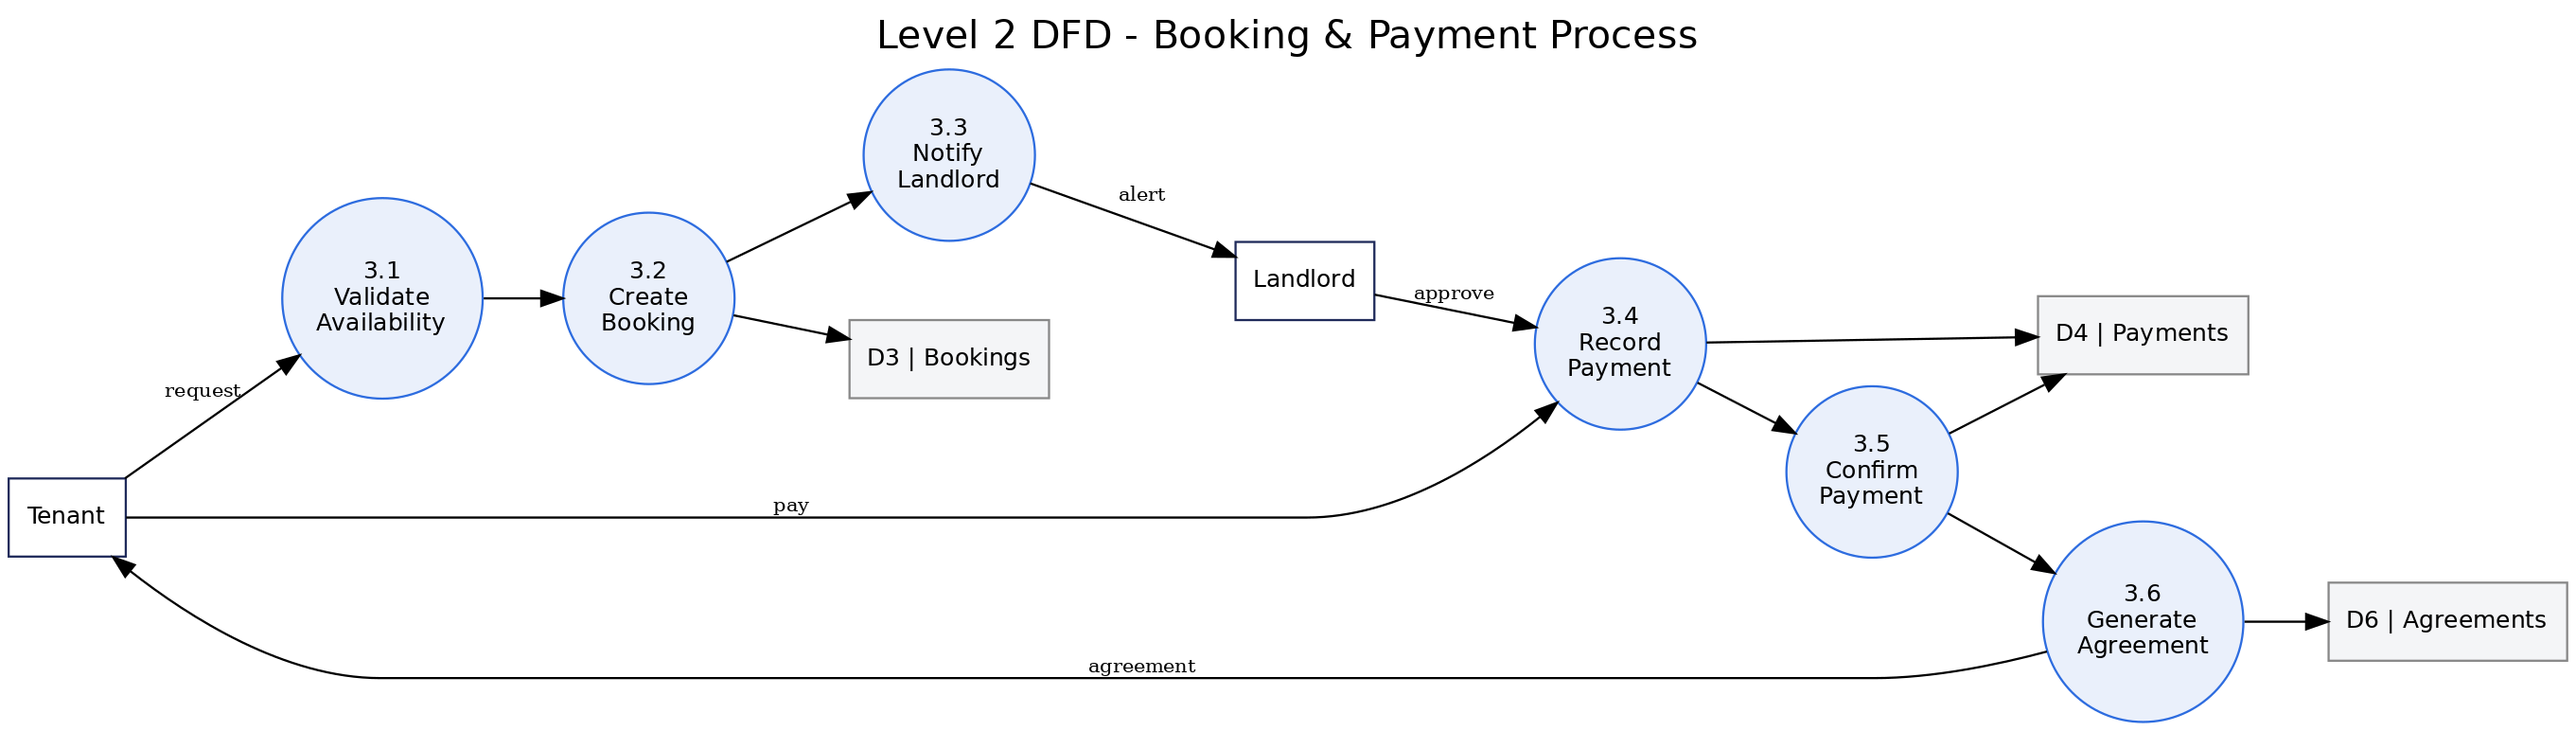
\includegraphics[width=0.9\textwidth]{Figures/DFD Sample 2.png}
\caption{Level 2 Data Flow Diagram (Sample)}
\label{fig:dfd2}
\end{figure}

The Level 2 DFD further decomposes the Booking and Payment process. It details the sub-processes of validating booking availability, creating the booking record, notifying the landlord, recording payment details, confirming payment, and triggering agreement generation, showing the data flowing into and out of the Bookings, Payments, and Agreements data stores at each step.

%%%%%%%%%%%%%%%%%%%%%%%%%%%%%%%%%%%%%%%%%%%%%%%%%%%%%%
\section{Data Design}

This section describes how data is structured, stored, and managed. Property Rental System uses MongoDB, a document-oriented NoSQL database, accessed through the Mongoose object data modelling library. The schema is organised into discrete collections that mirror the domain entities. Documents reference one another by ObjectId to model relationships, and indexes are defined on frequently queried fields, including a 2dsphere geospatial index on property location and compound indexes on status fields, to ensure efficient queries. Security mechanisms include password hashing, role-based access control, and restricted access to verification documents.

%%%%%%%%%%%%%%%%%%%%%%%%%%%%%%%%%%%%%%%%%%%%%%%%%%%%%%
\subsection{Entity Relationship Diagram (ERD)}

\begin{figure}[h]
\centering
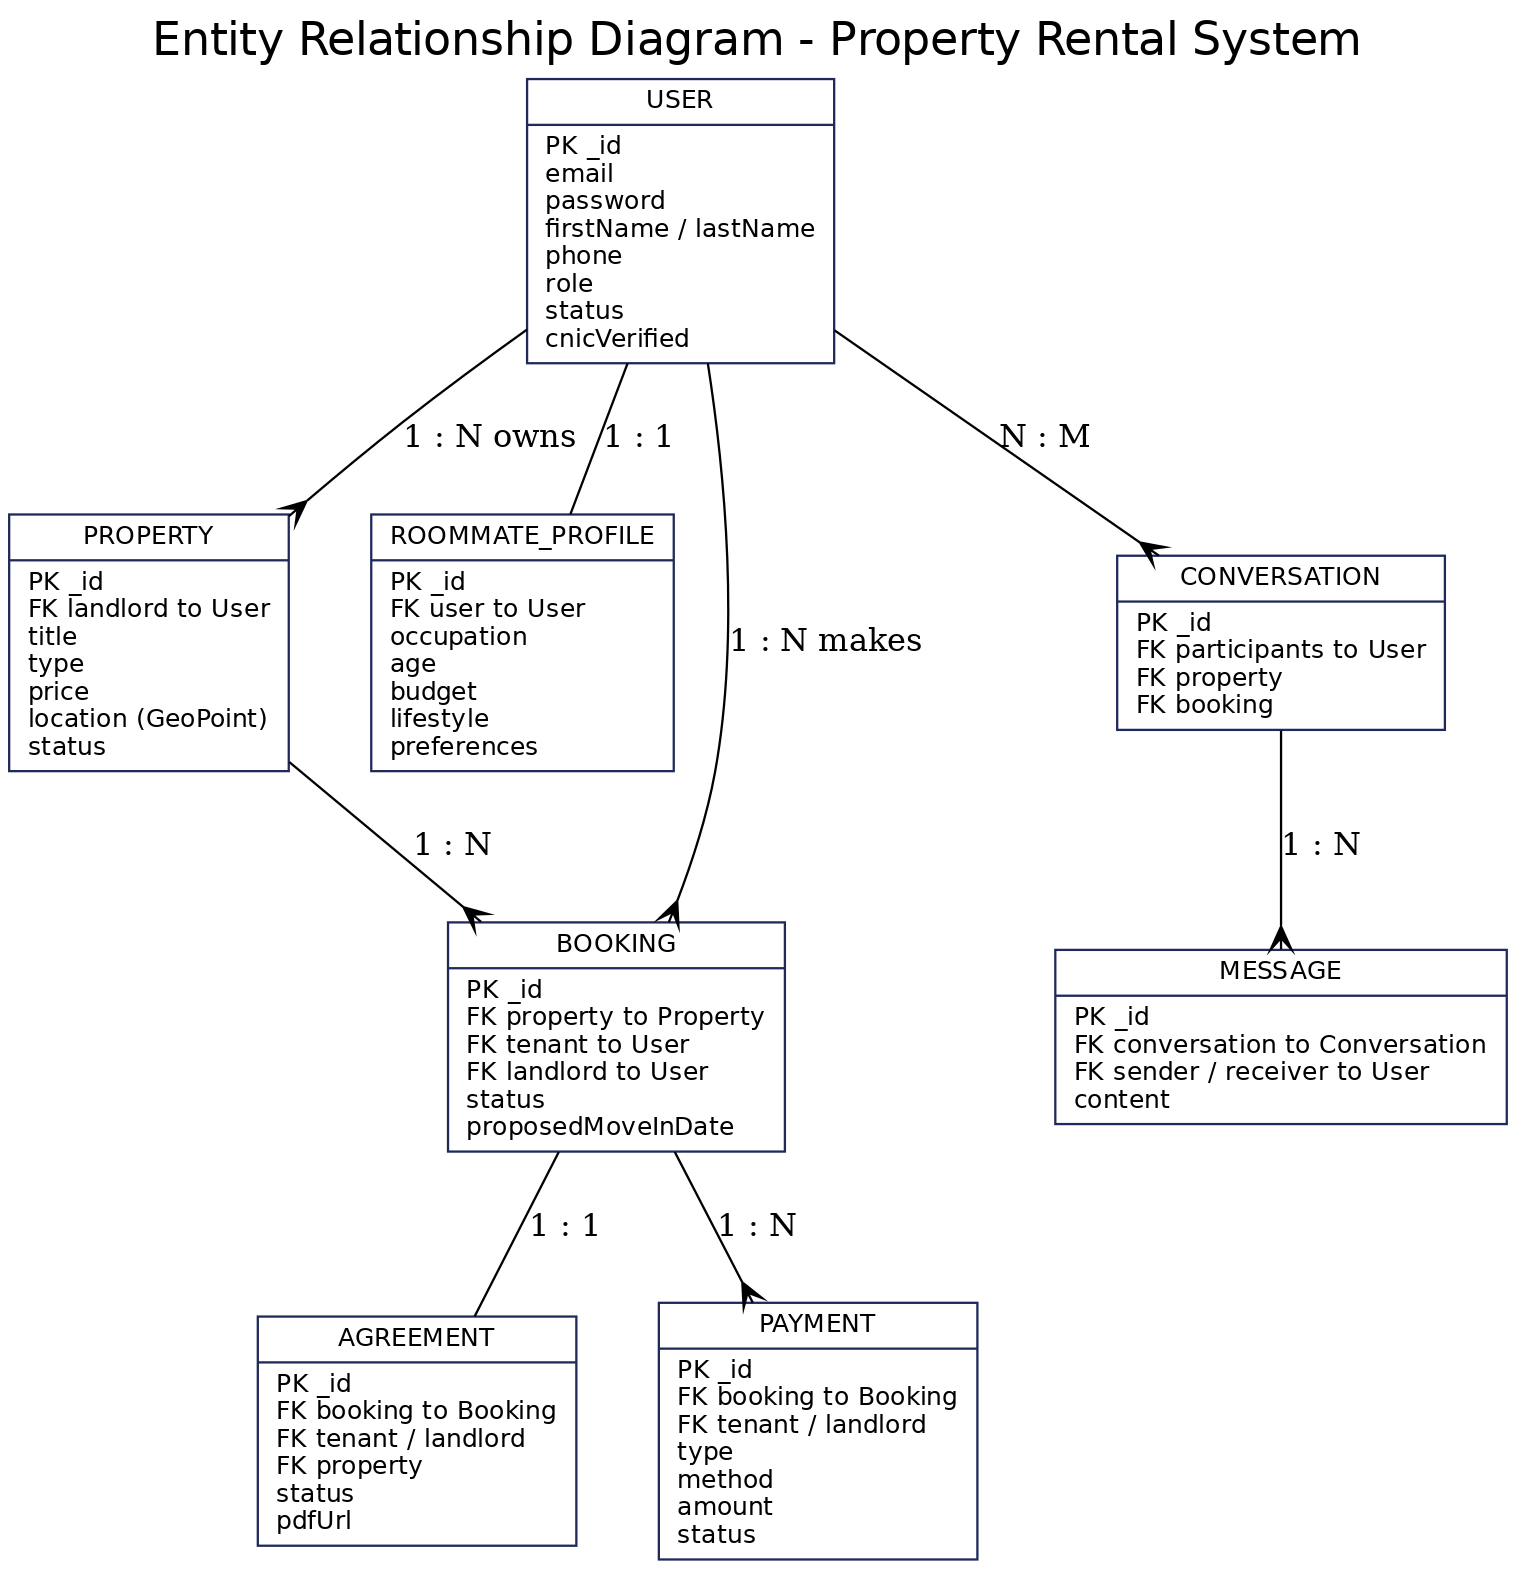
\includegraphics[width=0.9\textwidth]{Figures/ER Diagram.png}
\caption{Entity Relationship Diagram (Sample)}
\label{fig:erd}
\end{figure}

The ERD represents the logical structure of the Property Rental System database. The principal entities are User, Property, RoommateProfile, Booking, Agreement, Payment, Conversation, Message, Document, and LandlordBankAccount. A User (landlord) owns many Properties (1:N); a User (tenant) makes many Bookings (1:N); a Property has many Bookings (1:N); a Booking produces one Agreement (1:1) and one or more Payments (1:N); a Conversation contains many Messages (1:N) and links two Users; and a User has one RoommateProfile (1:1). \textit{(Replace the sample figure with the finalised Property Rental System ERD before submission.)}

%%%%%%%%%%%%%%%%%%%%%%%%%%%%%%%%%%%%%%%%%%%%%%%%%%%%%%
\subsection{Database Architecture}

Property Rental System uses a client-server database architecture in which the Express application server is the sole client of the MongoDB database. Property images and verification documents are stored in cloud media storage, with the database retaining only their secure references. This separation keeps the database lean and allows media to be served efficiently. The design supports cloud deployment and can be scaled through MongoDB replication and sharding if required.

%%%%%%%%%%%%%%%%%%%%%%%%%%%%%%%%%%%%%%%%%%%%%%%%%%%%%%
\section{Database Schema Diagram}

\begin{figure}[h]
\centering
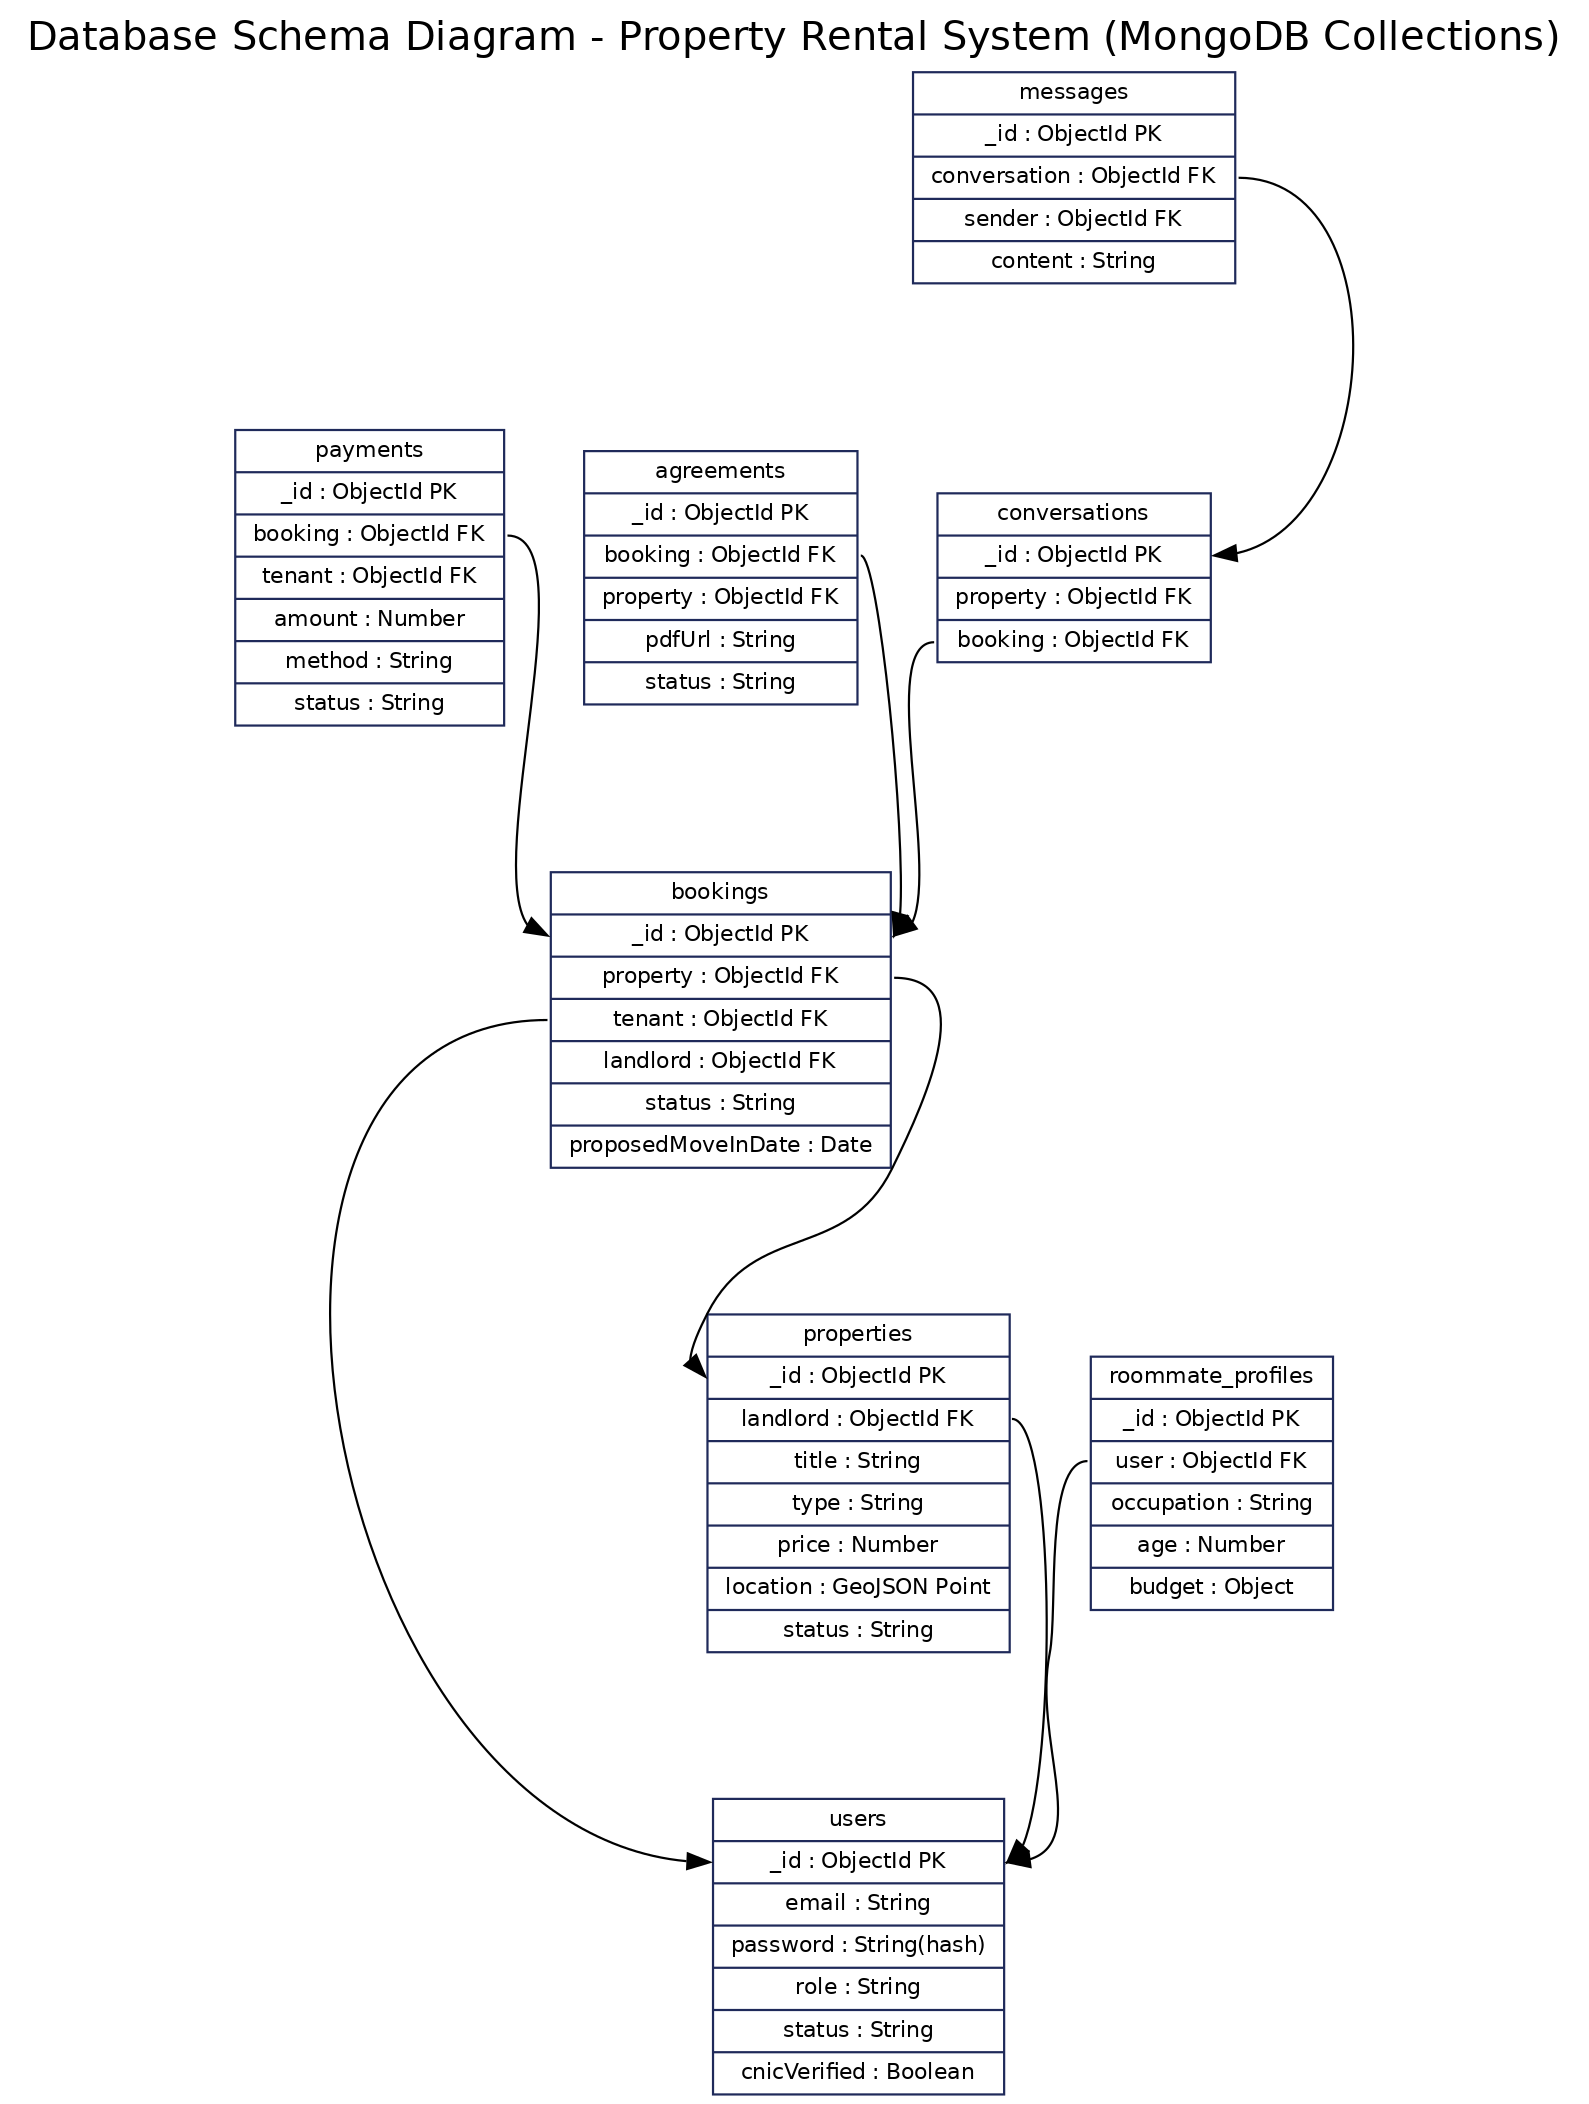
\includegraphics[width=0.9\textwidth]{Figures/Database Diagram.png}
\caption{Database Schema Diagram (Sample)}
\label{fig:dbschema}
\end{figure}

The schema diagram represents the physical structure of the collections, including field names, types, and the reference relationships between collections. The design supports data integrity through schema validation in Mongoose, efficient querying through indexing, scalability through a document model that avoids costly joins, and security through controlled access to sensitive fields. \textit{(Replace the sample figure with the finalised Property Rental System schema diagram.)}

%%%%%%%%%%%%%%%%%%%%%%%%%%%%%%%%%%%%%%%%%%%%%%%%%%%%%%
\subsection{Data Dictionary}

The data dictionary defines the structure of the principal data elements of the User collection as a representative example.

\begin{table}[h]
\centering
\caption{Data Dictionary -- User Collection}
\begin{tabularx}{\textwidth}{|p{3cm}|p{2.5cm}|X|}
\hline
\textbf{Field Name} & \textbf{Type} & \textbf{Description} \\
\hline
\_id & ObjectId & Unique identifier for each user \\
\hline
name & String & Full name of the user \\
\hline
email & String & Unique registered email address \\
\hline
passwordHash & String & Securely hashed password \\
\hline
role & String & User role: tenant, landlord, or admin \\
\hline
status & String & Account status: pending, active, or suspended \\
\hline
isVerified & Boolean & Indicates whether identity verification is complete \\
\hline
createdAt & Date & Account creation timestamp \\
\hline
\end{tabularx}
\end{table}

%%%%%%%%%%%%%%%%%%%%%%%%%%%%%%%%%%%%%%%%%%%%%%%%%%%%%%
%===========================================================
\section{Database Collections}
%===========================================================

This section describes the logical database design of Property Rental System. As a NoSQL system, the database is organised into collections, each modelling a domain entity with primary identifiers, references, and major attributes. The design ensures data consistency, integrity, security, and scalability.

%%%%%%%%%%%%%%%%%%%%%%%%%%%%%%%%%%%%%%%%%%%%%%%%%%%%%%
\subsection{User Collection}
%%%%%%%%%%%%%%%%%%%%%%%%%%%%%%%%%%%%%%%%%%%%%%%%%%%%%%

The User collection stores authentication credentials and profile information for all roles and supports role-based access control and secure authentication.

\begin{table}[h]
\centering
\caption{User Collection Structure}

\begin{tabularx}{\textwidth}{|p{3cm}|p{3cm}|p{3cm}|X|}
\hline
\textbf{Field Name} & \textbf{Data Type} & \textbf{Constraint} & \textbf{Description} \\
\hline
\_id & ObjectId & Primary Key & Unique identifier \\
\hline
name & String & Not Null & User's full name \\
\hline
email & String & Unique, Not Null & Login email address \\
\hline
passwordHash & String & Not Null & Hashed password \\
\hline
role & String & Not Null & tenant / landlord / admin \\
\hline
status & String & Default pending & Account status \\
\hline
createdAt & Date & Default now & Creation timestamp \\
\hline
\end{tabularx}

\end{table}

%%%%%%%%%%%%%%%%%%%%%%%%%%%%%%%%%%%%%%%%%%%%%%%%%%%%%%
\subsection{Property Collection}
%%%%%%%%%%%%%%%%%%%%%%%%%%%%%%%%%%%%%%%%%%%%%%%%%%%%%%

The Property collection stores micro-rental listings created by landlords, including location as a GeoJSON point to support geospatial search.

\begin{table}[h]
\centering
\caption{Property Collection Structure}

\begin{tabularx}{\textwidth}{|p{3cm}|p{3cm}|p{3cm}|X|}
\hline
\textbf{Field Name} & \textbf{Data Type} & \textbf{Constraint} & \textbf{Description} \\
\hline
\_id & ObjectId & Primary Key & Unique identifier \\
\hline
landlord & ObjectId & Foreign Key (User) & Owner of the listing \\
\hline
title & String & Not Null & Listing title \\
\hline
type & String & Not Null & room / bed space / hostel \\
\hline
price & Number & Not Null & Rent amount \\
\hline
location & GeoJSON Point & 2dsphere index & Geographic coordinates \\
\hline
status & String & Default pending\_verification & Listing status \\
\hline
\end{tabularx}

\end{table}

%%%%%%%%%%%%%%%%%%%%%%%%%%%%%%%%%%%%%%%%%%%%%%%%%%%%%%
\subsection{Booking, Payment, and Agreement Collections}
%%%%%%%%%%%%%%%%%%%%%%%%%%%%%%%%%%%%%%%%%%%%%%%%%%%%%%

The \textbf{Booking} collection records each rental request, referencing the tenant, landlord, and property, and tracking the booking status and move-in date. The \textbf{Payment} collection records payment type, method, amount, bank details, and status (pending or confirmed), referencing the related booking, tenant, and landlord. The \textbf{Agreement} collection stores the auto-generated rental agreement reference and terms for a confirmed booking. The \textbf{RoommateProfile} collection stores each user's lifestyle, preferences, budget, location, and schedule data along with cached compatibility scores. The \textbf{Conversation} and \textbf{Message} collections store in-app messaging, while \textbf{Document} and \textbf{LandlordBankAccount} store verification documents and landlord payout details respectively.

%%%%%%%%%%%%%%%%%%%%%%%%%%%%%%%%%%%%%%%%%%%%%%%%%%%%%%
\subsection{Relationships Between Collections}
%%%%%%%%%%%%%%%%%%%%%%%%%%%%%%%%%%%%%%%%%%%%%%%%%%%%%%

\begin{itemize}
    \item \textbf{One-to-One (1:1):} Each user has one roommate profile; each confirmed booking has one agreement.
    \item \textbf{One-to-Many (1:N):} A landlord owns many properties; a tenant makes many bookings; a property has many bookings; a conversation has many messages.
    \item \textbf{Many-to-Many (M:N):} Tenants interact with many properties through bookings and conversations, and properties are viewed by many tenants, resolved through the Booking and Conversation collections.
\end{itemize}

%%%%%%%%%%%%%%%%%%%%%%%%%%%%%%%%%%%%%%%%%%%%%%%%%%%%%%
\subsection{Security and Data Integrity}
%%%%%%%%%%%%%%%%%%%%%%%%%%%%%%%%%%%%%%%%%%%%%%%%%%%%%%

\begin{itemize}
    \item Password hashing using a secure algorithm (bcrypt) with salting.
    \item Role-based access control (RBAC) enforced through authentication middleware.
    \item Schema-level validation and constraints enforced by Mongoose.
    \item Secure communication over HTTPS and authenticated API requests via JWT.
    \item Restricted access to verification documents and regular database backups.
\end{itemize}

%%%%%%%%%%%%%%%%%%%%%%%%%%%%%%%%%%%%%%%%%%%%%%%%%%%%%%
\subsection{Scalability Considerations}
%%%%%%%%%%%%%%%%%%%%%%%%%%%%%%%%%%%%%%%%%%%%%%%%%%%%%%

\begin{itemize}
    \item Indexing on frequently queried attributes, including a geospatial index for location-based search.
    \item A document data model that avoids expensive joins and supports horizontal scaling.
    \item Offloading of media to cloud storage to keep the database lightweight.
    \item Support for MongoDB replication and sharding for future growth.
\end{itemize}

%%%%%%%%%%%%%%%%%%%%%%%%%%%%%%%%%%%%%%%%%%%%%%%%%%%%%%
\section{Chapter Summary}
%%%%%%%%%%%%%%%%%%%%%%%%%%%%%%%%%%%%%%%%%%%%%%%%%%%%%%

This chapter presented the comprehensive software design of the Property Rental System platform.
It justified an object-oriented, layered MVC design methodology and an Agile
process model, and described the system through a context diagram and a
three-layer client-server architecture. Detailed UML models, including activity,
class, sequence, and state transition diagrams, were developed to describe the
system's behaviour and structure, and data flow diagrams illustrated internal
data movement. The chapter further elaborated the database design through the
entity relationship model, schema diagram, data dictionary, and collection
specifications, addressing relationships, security, integrity, and scalability.
Overall, this chapter establishes a clear technical blueprint that guides the
implementation phase discussed in the next chapter.
